\documentclass[unicode,12pt,aspectratio=169,dvipdfmx]{beamer}
\usepackage{bxdpx-beamer}
\usetheme[progressbar=frametitle]{metropolis}
\renewcommand{\kanjifamilydefault}{\gtdefault}
\usepackage{bm}

\title{介護における音響HARと連合学習を用いた異常検知}
% \title{「A Survey on Federated Learning in Human Sensing」について}
\author{竹本志恩}
\institute{INIAD}
\date{\today}
\subject{研究報告 / 輪読}
\AtBeginSection[]{
  \begin{frame}[plain]
    \frametitle{目次}
    \tableofcontents[currentsection, hideallsubsections]
  \end{frame}
}

% --- セクション開始時に目次を表示 ---
\AtBeginSection[]{%
  \frame{\frametitle{目次}\tableofcontents[currentsection, hideallsubsections]}%
}

\begin{document}

% タイトルスライド
\begin{frame}
    \titlepage
\end{frame}

% 各セクション
\section{はじめに}

\begin{frame}{発表論文の概要}
  \begin{itemize}
    \item \textbf{タイトル:} A Survey on Federated Learning in Human Sensing
    \item \textbf{著者:} Mohan Li ほか
    \item \textbf{出典:} ACM, 2025年1月
    \item \textbf{内容:} Human Sensing分野におけるFederated Learning(FL)の包括的サーベイ
    \begin{itemize}
      \item 現状、課題、FLの分類、今後の研究方向を整理
    \end{itemize}
  \end{itemize}
\end{frame}

\begin{frame}{Human Sensingとは}
  \begin{itemize}
    \item 人の活動や生理・心理状態をセンサで監視し、生活の質向上などに貢献
    \item センサやウェアラブルデバイス進展により急速に普及
    \item 収集データは個人情報であり、プライバシーや倫理・法的課題が深刻
    \item このため\textbf{Federated Learning}によるプライバシー保護が期待される
  \end{itemize}
\end{frame}


\section{本サーベイの貢献と主要ドメイン}

\begin{frame}{本サーベイの貢献}
  \begin{itemize}
    \item Human Sensingに特化したFLサーベイ
    \item \textbf{8次元フレームワーク}の提案(主要な課題分析)
      \begin{itemize}
        \item プライバシー、セキュリティ、通信コスト、システム/統計的異質性など
      \end{itemize}
    \item 研究領域ごとの分類・まとめ
  \end{itemize}
\end{frame}


\begin{frame}{主要な応用ドメイン}
  \begin{columns}
    \begin{column}[T]{0.65\linewidth}
      \begin{itemize}
        \item Human Sensing分野でのFL応用を6分野に分類
        \item \textbf{Activity Recognition (HAR)} が31.6\%と最多
        \item Well-being、User Identificationなどが続く
        \item Interface Developmentは最小(3.3\%)
        \item \textbf{HAR}は注目分野
      \end{itemize}
    \end{column}
    \begin{column}[T]{0.35\linewidth}
      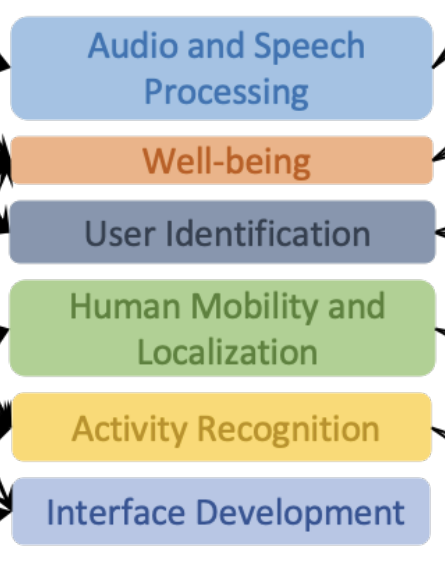
\includegraphics[width=\linewidth]{figures/対象の分野.png}
    \end{column}
  \end{columns}
\end{frame}

\begin{frame}{Fig.5}
    \center 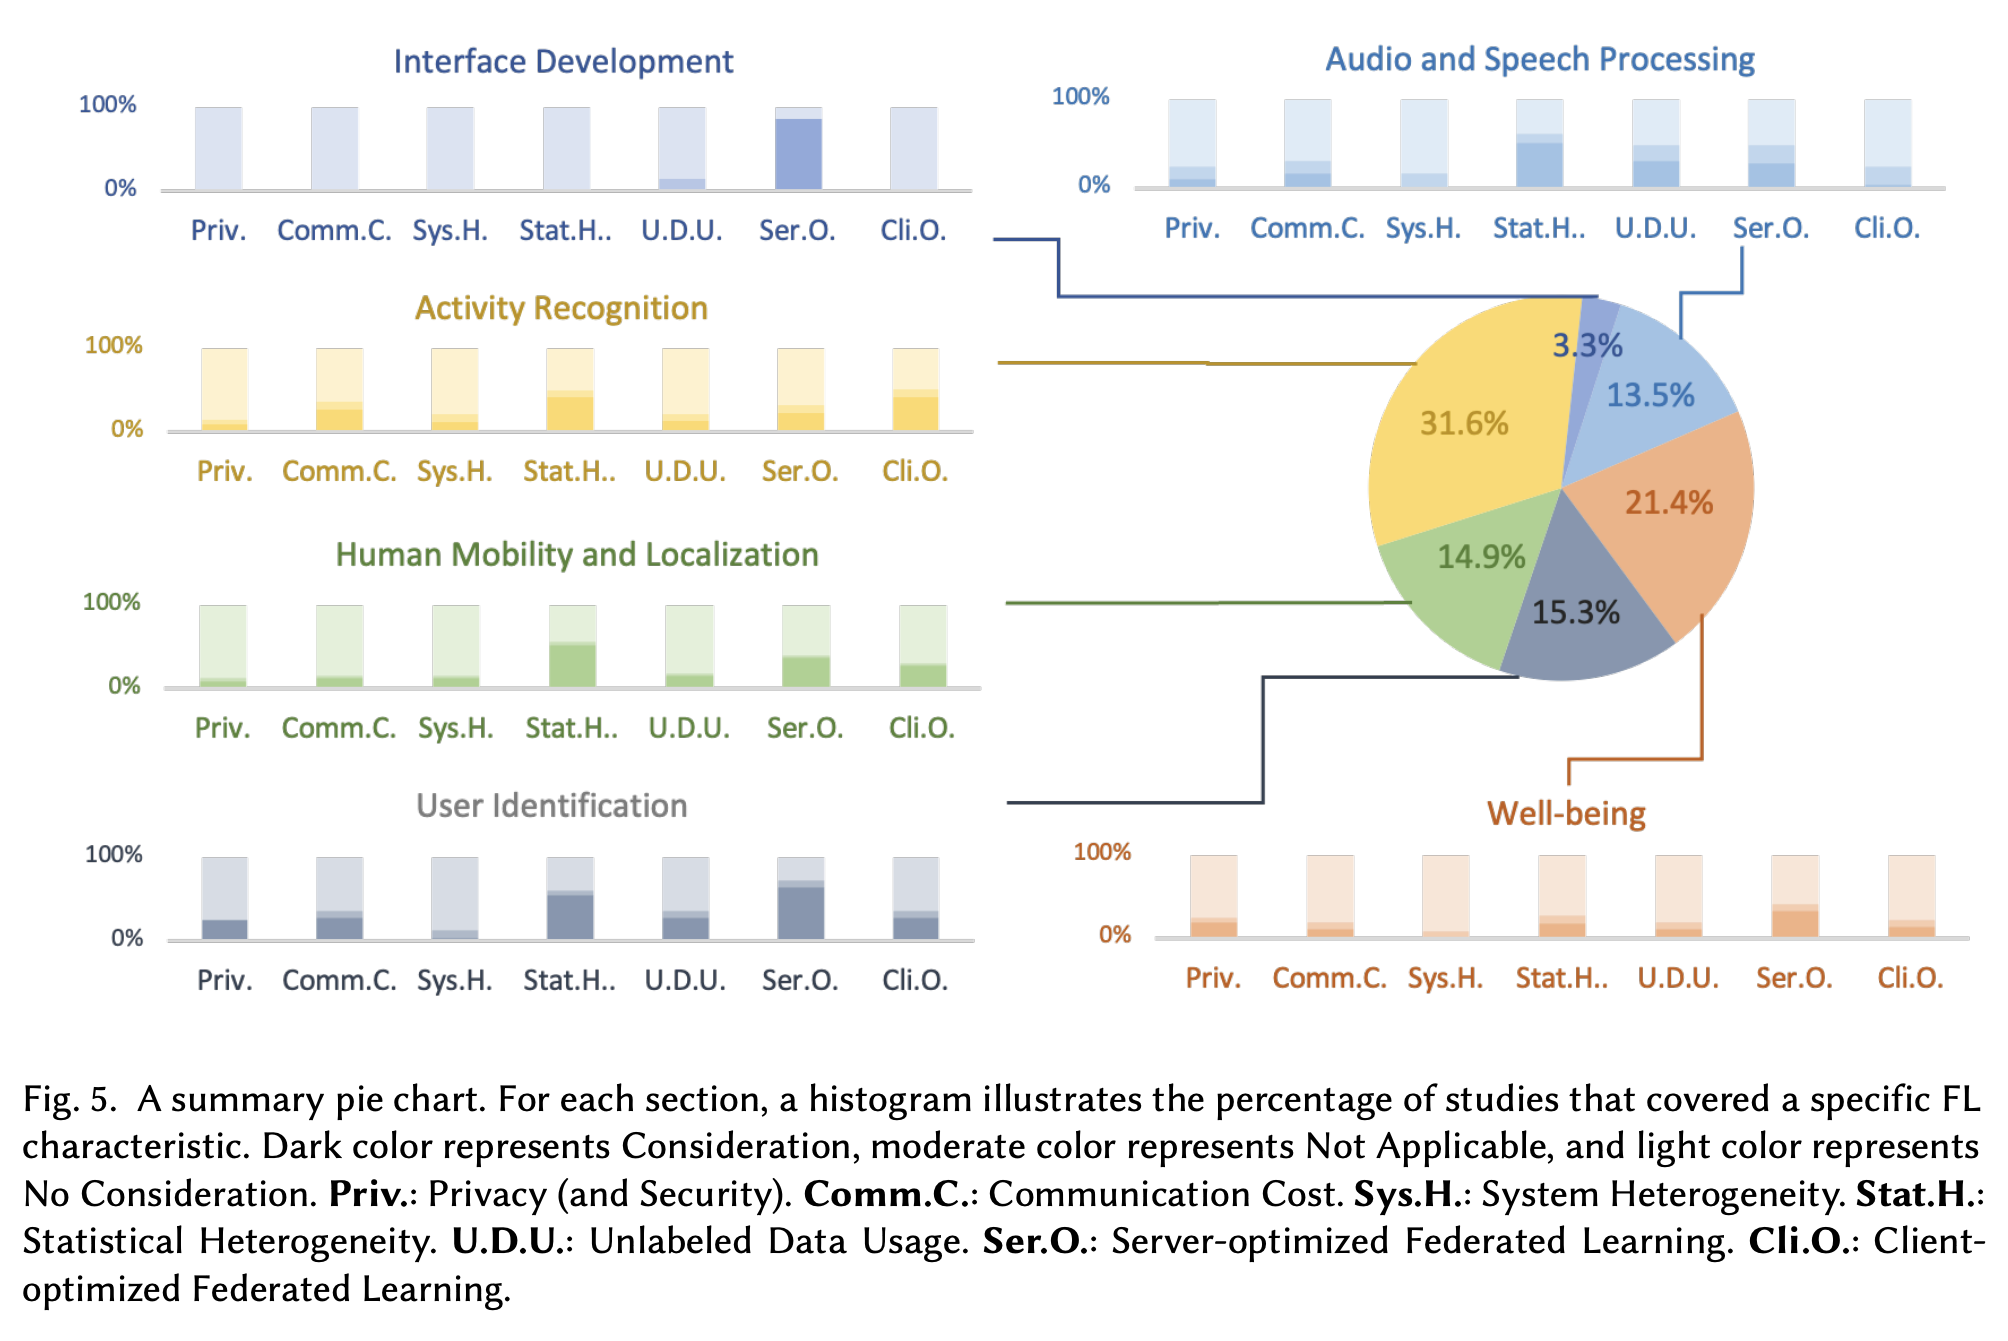
\includegraphics[scale=0.3]{figures/domain_per.png}                    
\end{frame}


\section{Human Activity Recognition (HAR) とは}

\begin{frame}{Human Activity Recognition (HAR) とは}
  \begin{itemize}
    \item センサデータから人の活動を自動認識する技術
    \item 応用例:ヘルスケア、スマートホーム、リハビリ、転倒検知
    \item 主要なセンサ
      \begin{itemize}
        \item \textbf{ウェアラブル:} スマートウォッチ・スマホ等(加速度・ジャイロ)
        \item \textbf{環境:} マイク、圧力センサ等(非装着型)
        \item \textbf{カメラ:} 高精度だがプライバシー懸念が大きい
      \end{itemize}
  \end{itemize}
\end{frame}

\begin{frame}{HARの課題}
  \begin{itemize}
    \item \textbf{プライバシー懸念:} カメラや中央集権型データ収集のリスク
    \item \textbf{通信コスト:} 大量データの転送負担
    \item \textbf{データセット不足:} プライバシー規制で大規模実験困難
  \end{itemize}
\end{frame}



\section{HARにおけるFLの導入と想定シナリオ}

\begin{frame}{HARにおけるFLの導入}
  \begin{itemize}
    \item \textbf{プライバシー保護:} モデルパラメータのみ共有し、生データはローカル保持
    \item \textbf{通信コスト削減:} 軽量なパラメータ通信
    \item \textbf{分散型:} 中央集権的データ転送が不要
    \item Non-IID(各クライアントのデータ分布が異なる)等の現実課題
  \end{itemize}
\end{frame}

\begin{frame}{介護施設での見守りシステム:シナリオ}
  \begin{itemize}
    \item \textbf{目的:} 異常(転倒・咳込み・苦痛など)の早期検知・通知
    \item \textbf{背景:} 高齢化&介護人材不足、安価&高精度なシステム需要
    \item \textbf{技術構成:}
      \begin{itemize}
        \item 音響HAR:各部屋IoTマイクで環境音取得・分類
        \item 行動認識:時系列・音響イベントから状態判断
        \item Federated Learning:部屋ごとローカル学習+全体モデル更新
      \end{itemize}
  \end{itemize}
\end{frame}

\begin{frame}{FL導入の利点(介護シナリオ)}
  \begin{itemize}
    \item \textbf{プライバシー保護:} 生音声は部屋内ローカルでのみ処理
    \item \textbf{パーソナル化:} 利用者/部屋ごとのモデル最適化が可能
  \end{itemize}
\end{frame}


\begin{frame}{想定される課題と検討}
  \begin{itemize}
    \item \textbf{緊急イベントのデータ不足:} 稀なため収集困難
      \begin{itemize}
        \item Openデータや合成データで対応
      \end{itemize}
    \item \textbf{データ異質性(Non-IID):} 部屋・利用者ごとに環境・頻度が違う
    \item \textbf{クライアント異質性:} デバイス能力差あり → 軽量モデルや部分学習で対応
  \end{itemize}
\end{frame}

\begin{frame}{さらなる課題}
  \begin{itemize}
    \item \textbf{リアルタイム性:} 異常検知は即時対応が必要、通信・推論レイテンシを考慮
    \item \textbf{モデル汎化性能:} 新規利用者・環境にも適用可能か(メタラーニング、表現学習)
  \end{itemize}
\end{frame}


\section{HAR-FLの主要課題とFLの対応(サーベイより)}

\begin{frame}{主要な課題とFLの対応}
  \begin{itemize}
    \item \textbf{データ異質性(Non-IID)}:
      \begin{itemize}
        \item 従来のFedAvgは性能劣化
        \item \textbf{パーソナル化FL}、クラスタリング、知識蒸留等で対応
      \end{itemize}
    \item \textbf{ラベルデータ不足}:
      \begin{itemize}
        \item 半教師ありFL・自己教師あり学習で対応
      \end{itemize}
    \item \textbf{通信コスト}:
      \begin{itemize}
        \item モデル圧縮・FedDL(動的レイヤー共有)ほか
      \end{itemize}
    \item \textbf{プライバシー/セキュリティ}:DP・セキュアアグリゲーション
    \item \textbf{システム異質性}:リソースアウェアな手法
  \end{itemize}
\end{frame}

\section{まとめ}
\begin{frame}{まとめ}
  \begin{itemize}
    \item Human Sensingの普及には\textbf{データプライバシー課題}が障害
    \item Federated Learningはその解決策として有望
    \item HARはFL応用が特に活発な分野
  \end{itemize}
\end{frame}

\begin{frame}{今後の展望}
  \begin{itemize}
    \item 介護施設等での\textbf{プライバシ保護+高精度異常検知}の社会実装が期待
    \item 複数モダリティ統合、現場実験、プライバシー技術の進展
    \item HAR-FLのさらなる研究と社会実装に注目
  \end{itemize}
\end{frame}

\end{document}